\chapter{Implementación}

Neste capítulo se comentarán os aspectos máis relevantes da implementación da nosa plataforma, ben sexa polo uso de librerías externas ou porque requiriron un desenvolvemento especial. Farase mención a detalles do servidor, da aplicación Android así como da autenticación a través de Google.


\section{Servidor}
Nesta sección vanse tratar todos os detalles de implementación propios do servidor, dende o acceso á base de datos ata a construción dos servizos web. En todo o servidor utilizouse a ferramenta de Spring para configurar a transaccionalidade, a inxección de dependencias ou a creación dos servizos web.

A autenticación con Google terá a súa propia sección ao final do capítulo.


AWS.

\subsection{Acceso á base de datos}
Para o acceso á base de datos utilizouse directamente JDBC sen facer uso de ningunha ferramenta de mapeo obxecto-relacional como pode ser Hibernate. Escolleuse esta opción por ser un sistema sen moita complexidade á hora de gardar ou eliminar rexistros en base de datos e cun número de táboas non moi alto. En sistemas pequenos non se aproveitan os beneficios que poden ter estas ferramentas e desta maneira afórrase a súa configuración.

Creouse unha implementación para cada un dos DAOs amosados na sección de deseño. Dentro deles fanse todas as accións permitidas sobre as táboas que representa cada VO.

Exemplo de inxección de consulta

Exemplo de execución de consulta

\begin{figure}[tbh] 
	\begin{center}
		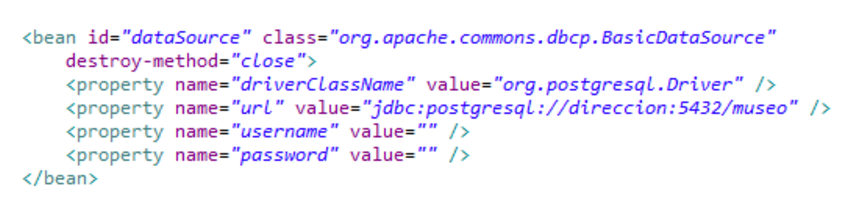
\includegraphics[width=1\textwidth]{figures/codigo/configuracionBD}
		\caption{Configuración da base de datos no ficheiro XML.}
		\label{fig:configuracionBD}
	\end{center}
\end{figure}

\begin{figure}[tbh] 
	\begin{center}
		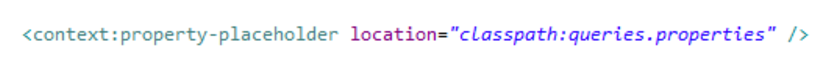
\includegraphics[width=1\textwidth]{figures/codigo/placeholderConsultas}
		\caption{Configuración en XML para a localización do ficheiro das consultas.}
		\label{fig:placeholderConsultas}
	\end{center}
\end{figure}

\begin{figure}[tbh] 
	\begin{center}
		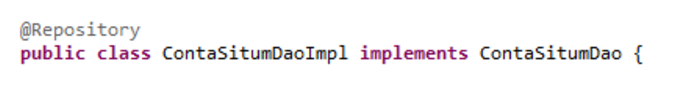
\includegraphics[width=1\textwidth]{figures/codigo/dao}
		\caption{Clase de implementación dun DAO.}
		\label{fig:dao}
	\end{center}
\end{figure}

\begin{figure}[tbh] 
	\begin{center}
		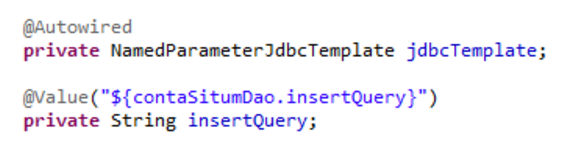
\includegraphics[width=1\textwidth]{figures/codigo/inxeccionDao}
		\caption{Inxección dunha consulta nun DAO.}
		\label{fig:inxeccionDao}
	\end{center}
\end{figure}

\begin{figure}[tbh] 
	\begin{center}
		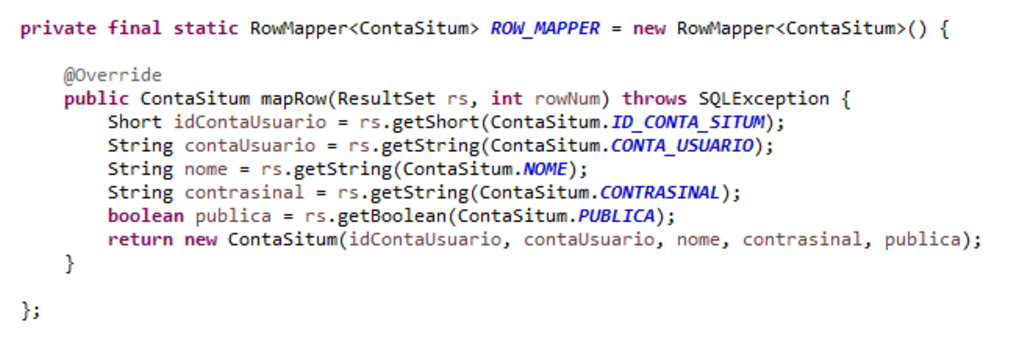
\includegraphics[width=1\textwidth]{figures/codigo/daoRowMapper}
		\caption{Construción dun VO dentro do DAO.}
		\label{fig:daoRowMapper}
	\end{center}
\end{figure}

\begin{figure}[tbh] 
	\begin{center}
		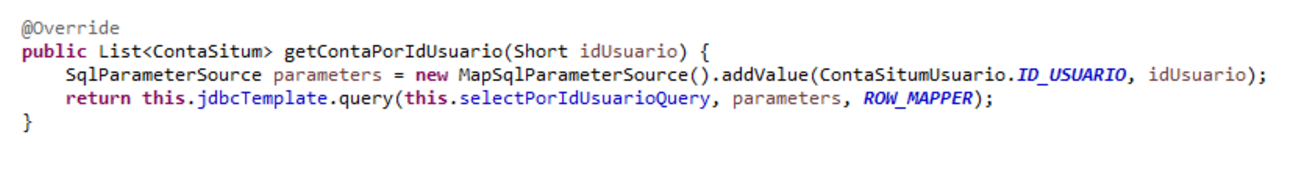
\includegraphics[width=1\textwidth]{figures/codigo/daoConsulta}
		\caption{Método de consulta dun DAO.}
		\label{fig:daoConsulta}
	\end{center}
\end{figure}

\begin{figure}[tbh] 
	\begin{center}
		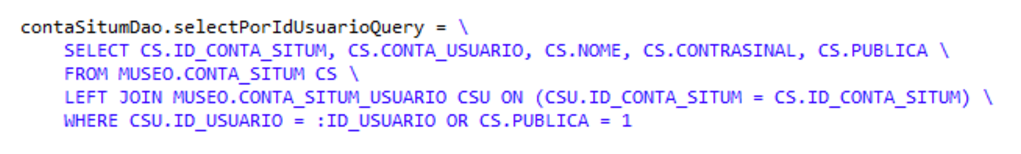
\includegraphics[width=1\textwidth]{figures/codigo/daoConsultaSQL}
		\caption{Exemplo dunha consulta en SQL.}
		\label{fig:daoConsultaSQL}
	\end{center}
\end{figure}

\begin{figure}[tbh] 
	\begin{center}
		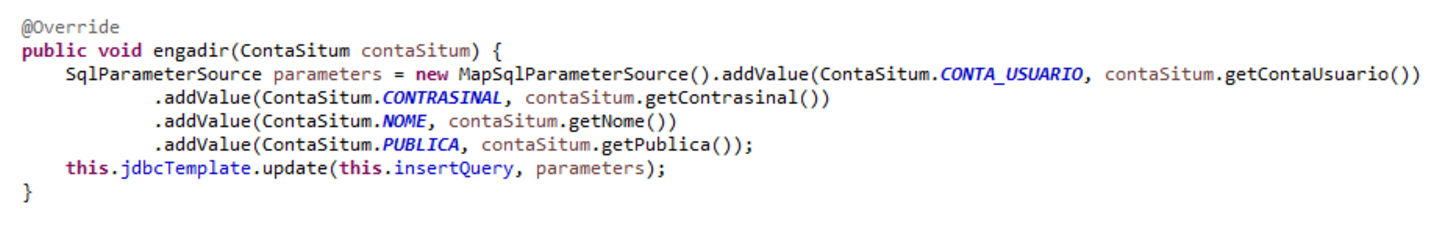
\includegraphics[width=1\textwidth]{figures/codigo/daoInsert}
		\caption{Método de inserción dun DAO.}
		\label{fig:daoInsert}
	\end{center}
\end{figure}

\begin{figure}[tbh] 
	\begin{center}
		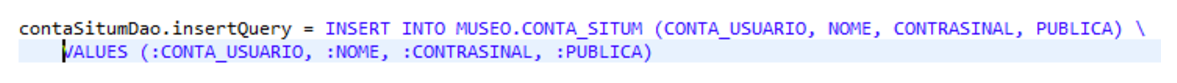
\includegraphics[width=1\textwidth]{figures/codigo/daoInsertSQL}
		\caption{Exemplo dunha inserción en SQL.}
		\label{fig:daoInsertSQL}
	\end{center}
\end{figure}










\subsection{Transaccionalidade}
A xestión transaccionalidade impleméntase na capa Manager utilizando o framework Spring, grazas á súa librería spring-tx. A súa configuración e utilización é moi sinxela, tal e como se pode observar nos exemplos. No primeiro amósase a configuración que require nos ficheiros XML de Spring. Para indicar a transaccionalidade, utilizaremos etiquetas que permitan identificar o tipo de transacción que queremos que se aplique en cada método público do manager. Non todos os métodos provocan escrituras en base de datos, polo que non será necesario indicar o tipo de transaccionalidade que provoca desfacer cambios en todos eles. O resto marcaranse como de só lectura para non sobrecargar innecesariamente o sistema.

Na figura~\ref{fig:transaccionConfiguracion} pódese observar a configuración da transaccionalidade nos ficheiros XML.

\begin{figure}[tbh] 
	\begin{center}
		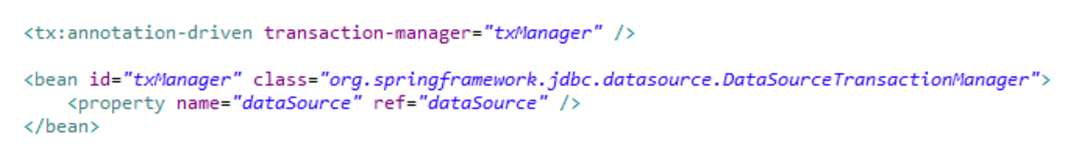
\includegraphics[width=1\textwidth]{figures/codigo/transaccionConfiguracion}
		\caption{Configuración da transaccionalidade no ficheiro XML.}
		\label{fig:transaccionConfiguracion}
	\end{center}
\end{figure}


Na figura~\ref{fig:metodoTransaccional} pódese observar a configuración da transaccionalidade sobre un método no que se modifican datos.

\begin{figure}[tbh] 
	\begin{center}
		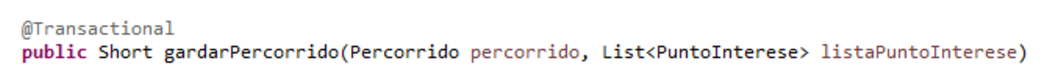
\includegraphics[width=1\textwidth]{figures/codigo/metodoTransaccional}
		\caption{Configuración da transaccionalidade dun método onde se modifican datos.}
		\label{fig:metodoTransaccional}
	\end{center}
\end{figure}

Na figura~\ref{fig:metodoNonTransaccional} pódese observar a configuración da transaccionalidade sobre un método de só lectura.

\begin{figure}[tbh] 
	\begin{center}
		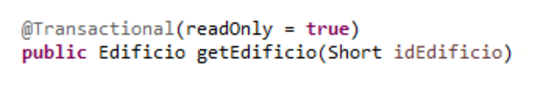
\includegraphics[width=0.5\textwidth]{figures/codigo/metodoNonTransaccional}
		\caption{Configuración da transaccionalidade dun método de só lectura.}
		\label{fig:metodoNonTransaccional}
	\end{center}
\end{figure}


\subsection{Construción dos servizos web}
Para a construción dos servizos web creáronse dous controladores distintos, tal e como se comentou na sección de deseño: un para as imaxes e o outro para o resto de información. Esta capa comúnicase coa capa dos manager, detallada na subsección anterior \todo{ligazon?}. Para a súa implementación usouse unha librería específica de Spring para a construción de servizos web: Spring MVC.


Exemplo de construción dos servizos web: Spring MVC
\begin{figure}[tbh] 
	\begin{center}
		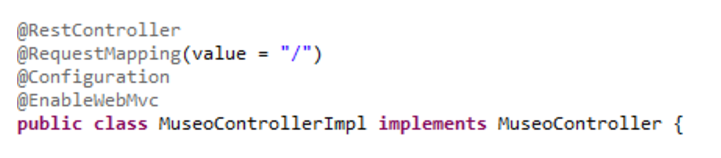
\includegraphics[width=0.5\textwidth]{figures/codigo/controladorMuseo}
		\caption{Exemplo de etiquetas sobre o servizo.}
		\label{fig:controladorMuseo}
	\end{center}
\end{figure}

\begin{figure}[tbh] 
	\begin{center}
		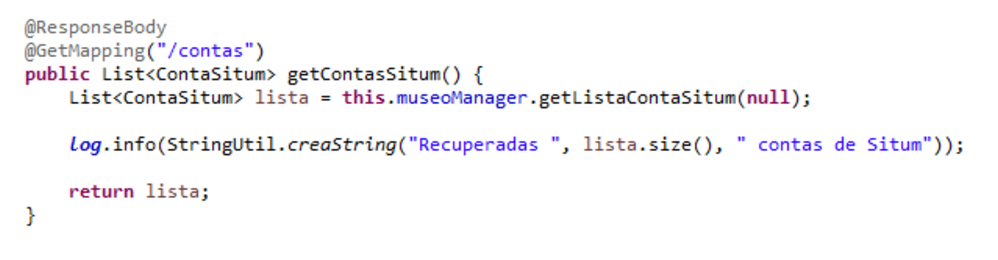
\includegraphics[width=0.5\textwidth]{figures/codigo/chamadaServizoGetSimple}
		\caption{Exemplo de método Get do servizo.}
		\label{fig:chamadaServizoGetSimple}
	\end{center}
\end{figure}

\begin{figure}[tbh] 
	\begin{center}
		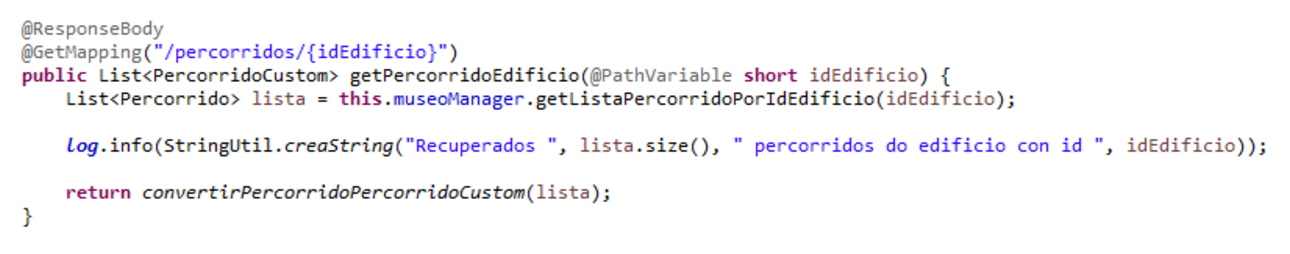
\includegraphics[width=0.5\textwidth]{figures/codigo/chamadaServizoGetParametro}
		\caption{Exemplo de método Get con parámetro do servizo.}
		\label{fig:chamadaServizoGetParametro}
	\end{center}
\end{figure}

\begin{figure}[tbh] 
	\begin{center}
		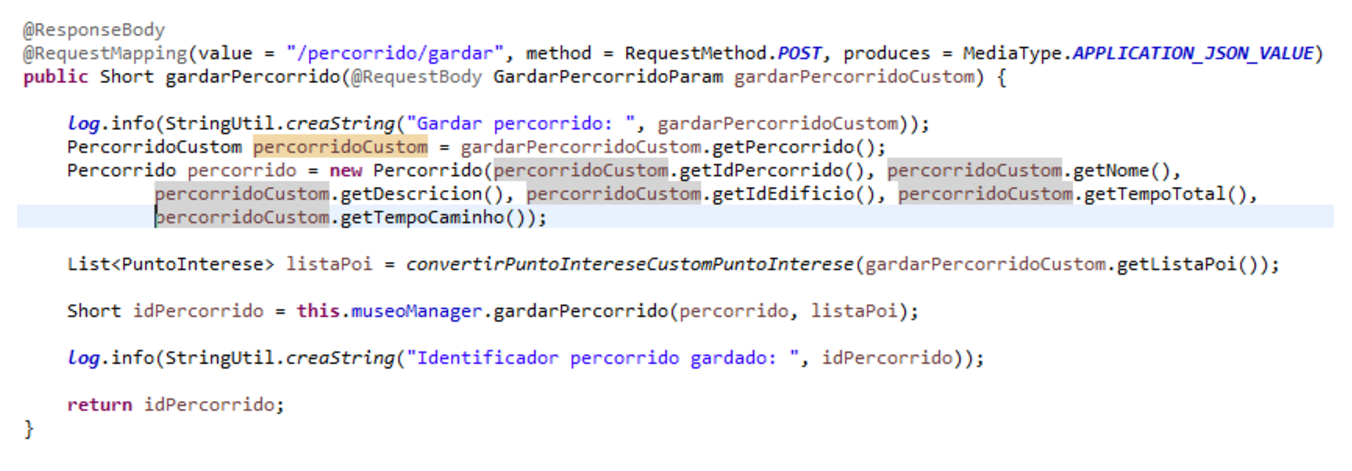
\includegraphics[width=0.5\textwidth]{figures/codigo/chamadaServizoPost}
		\caption{Exemplo de método Post do servizo.}
		\label{fig:chamadaServizoPost}
	\end{center}
\end{figure}

\begin{figure}[tbh] 
	\begin{center}
		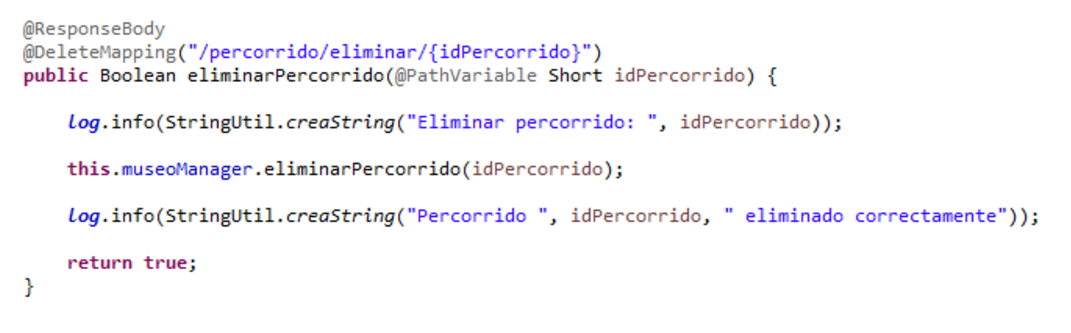
\includegraphics[width=0.5\textwidth]{figures/codigo/chamadaServizoDelete}
		\caption{Exemplo de método Delete do servizo.}
		\label{fig:chamadaServizoDelete}
	\end{center}
\end{figure}







\subsection{Autorización nos servizos}
Tal e como se indicou no apartado de deseño de "Securización das comunicacións", implementouse un sistema de autenticación básica sobre os servizos web, de tal maneira que non se permite a chamada a eses servizos se non se inclúe na cabeceira un token para a autenticación. Este token constrúese mediante a codificación en Base64 dun nome de usuario e contrasinal que son comúns ás chamadas. A configuración desta securización realízase no ficheiro web.xml, onde se inclúe o código da figura~\ref{fig:configuracionAutenticacion}.

\begin{figure}[htb] 
	\begin{center}
		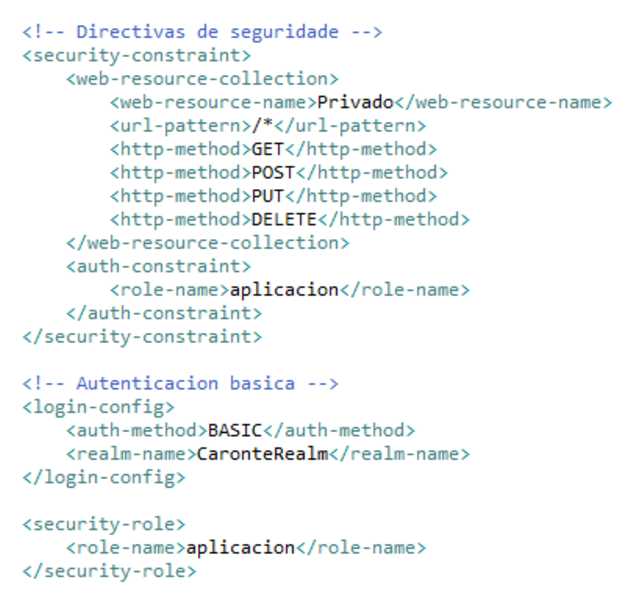
\includegraphics[width=0.6\textwidth]{figures/codigo/configuracionAutenticacion}
		\caption{Configuración da autenticación básica no servidor.}
		\label{fig:configuracionAutenticacion}
	\end{center}
\end{figure}

Como se pode observar na figura, securízanse as chamadas GET, DELETE, POST e PUT, que son as básicas nos servizos REST. Calquera chamada que non teña o token de autenticación correcto será rexeitada sen entrar no servizo.


\section{Aplicación Android}
Nesta sección trataranse os aspectos máis importantes da implementación na aplicación Android.
\subsection{Solicitude de permisos}
Como se solicitan permisos na aplicación
Non fan falla na instalación. Solicítanse na execución. Sen o permiso de localización non funcionaría a aplicación.

\subsection{Acceso a Situm}
Para o acceso aos servizos de Situm optouse por illar as conexións en clases distintas para non mesturar lóxica. Estes accesos realizáronse mediante o uso da SDK de Situm na súa versión \todo{mirar versión}.

Exemplo de acceso a Situm

\subsection{Acceso ao servidor}
Ao igual que se explicou no punto anterior, a conexión co servidor propio realizouse mediante conexións illadas en distintas clases. 
Exemplo de acceso ao servizo web




Exemplo de chamada a actividade e devolución do fluxo






\section{Autenticación}
Neste punto verase o proceso de autenticación en máis profundidade, revisando as diferentes chamadas necesarias tanto dende a aplicacion Android coma dende o servidor contra os servizos de Google para verificar a identidade do usuario.

O primeiro punto a ter en conta é a configuración necesaria para permitir a autenticación dende a aplicación. Débese incluir a dependencia con \emph{'com.google.android.gms:play-services-auth:12.0.1'} no build.gradle a nivel de aplicación e incluír o ficheiro google-services.json específico de Caronte que se pode conseguir despois de dar de alta o proxecto na consola de desenvolvemento de Google. Dende esta mesma consola pódense conseguir as credenciais que permiten a conexión cos servizos de Google que utilizaremos a continuación, na conexión dende a aplicación Android e dende o servidor.


\todo{https://console.developers.google.com/apis/credentials}

\todo{incluir referencia a https://developers.google.com/identity/sign-in/android/start-integrating}

\todo{https://developers.google.com/android/guides/client-auth}

\begin{figure}[htb] 
	\begin{center}
		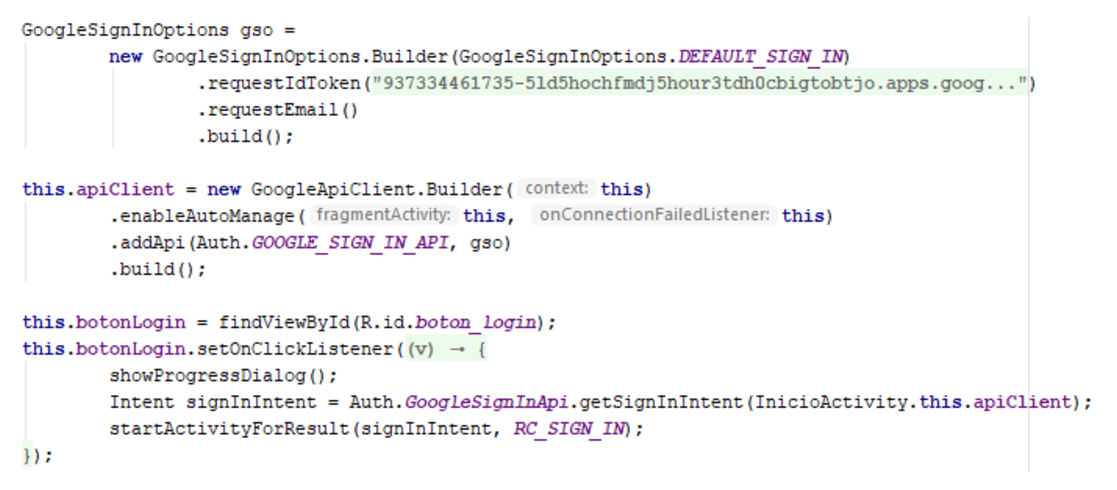
\includegraphics[width=0.9\textwidth]{figures/codigo/autenticacionGoogleInicio}
		\caption{Código para a autenticación con Google na aplicación.}
		\label{fig:autenticacionGoogleInicio}
	\end{center}
\end{figure}

O primeiro paso para permitir o acceso a un usuario concreto na aplicación é a obtención das credenciais de autenticación do usuario. Para lograr isto, temos o código da figura~\ref{fig:autenticacionGoogleInicio}. Pulsando sobre o botón de login lanzarase unha actividade propia de Google que permite a autenticación dentro da aplicación cunha conta de Google.

\begin{figure}[htb] 
	\begin{center}
		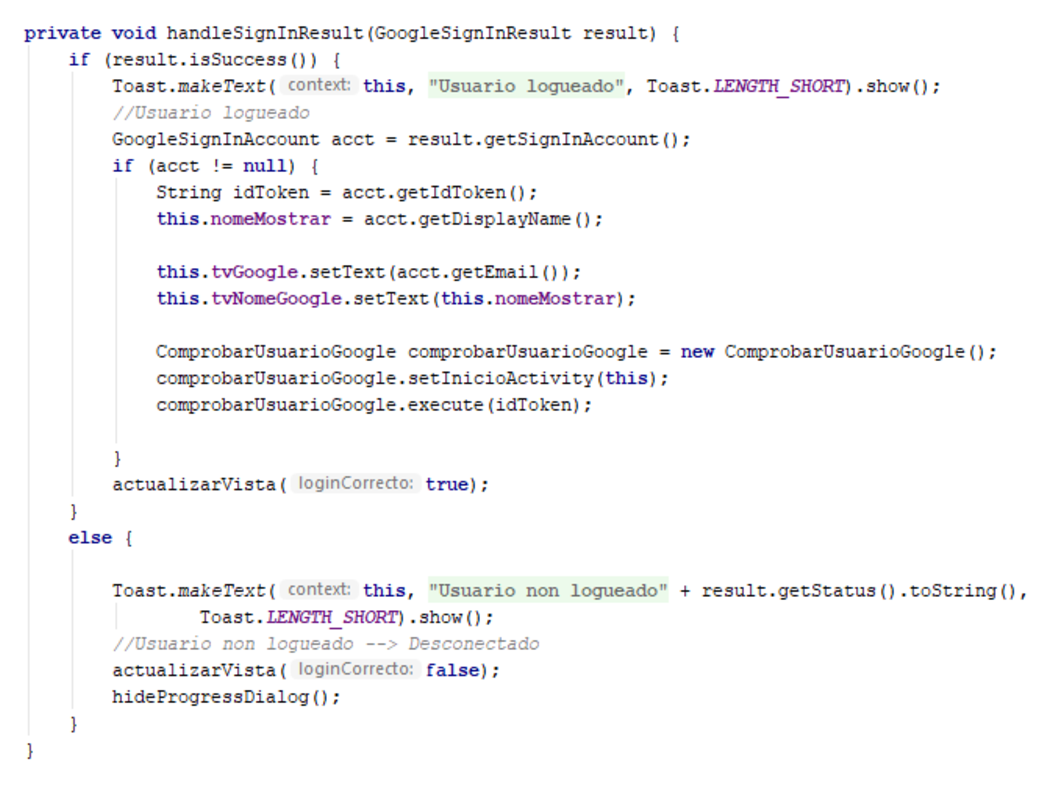
\includegraphics[width=0.9\textwidth]{figures/codigo/autenticacionGoogleRecepcion}
		\caption{Código para a autenticación con Google na aplicación (2).}
		\label{fig:autenticacionGoogleRecepcion}
	\end{center}
\end{figure}

O seguinte paso será o tratamento da información recibida cando a actividade lanzada no punto anterior remate correctamente. Pódese ver na figura~\ref{fig:autenticacionGoogleRecepcion} o tratamento dos datos. O punto principal é o lanzamento dunha chamada ao servidor de Caronte pasando como parametro un token enviado por Google para verificar a conta.

\begin{figure}[htb] 
	\begin{center}
		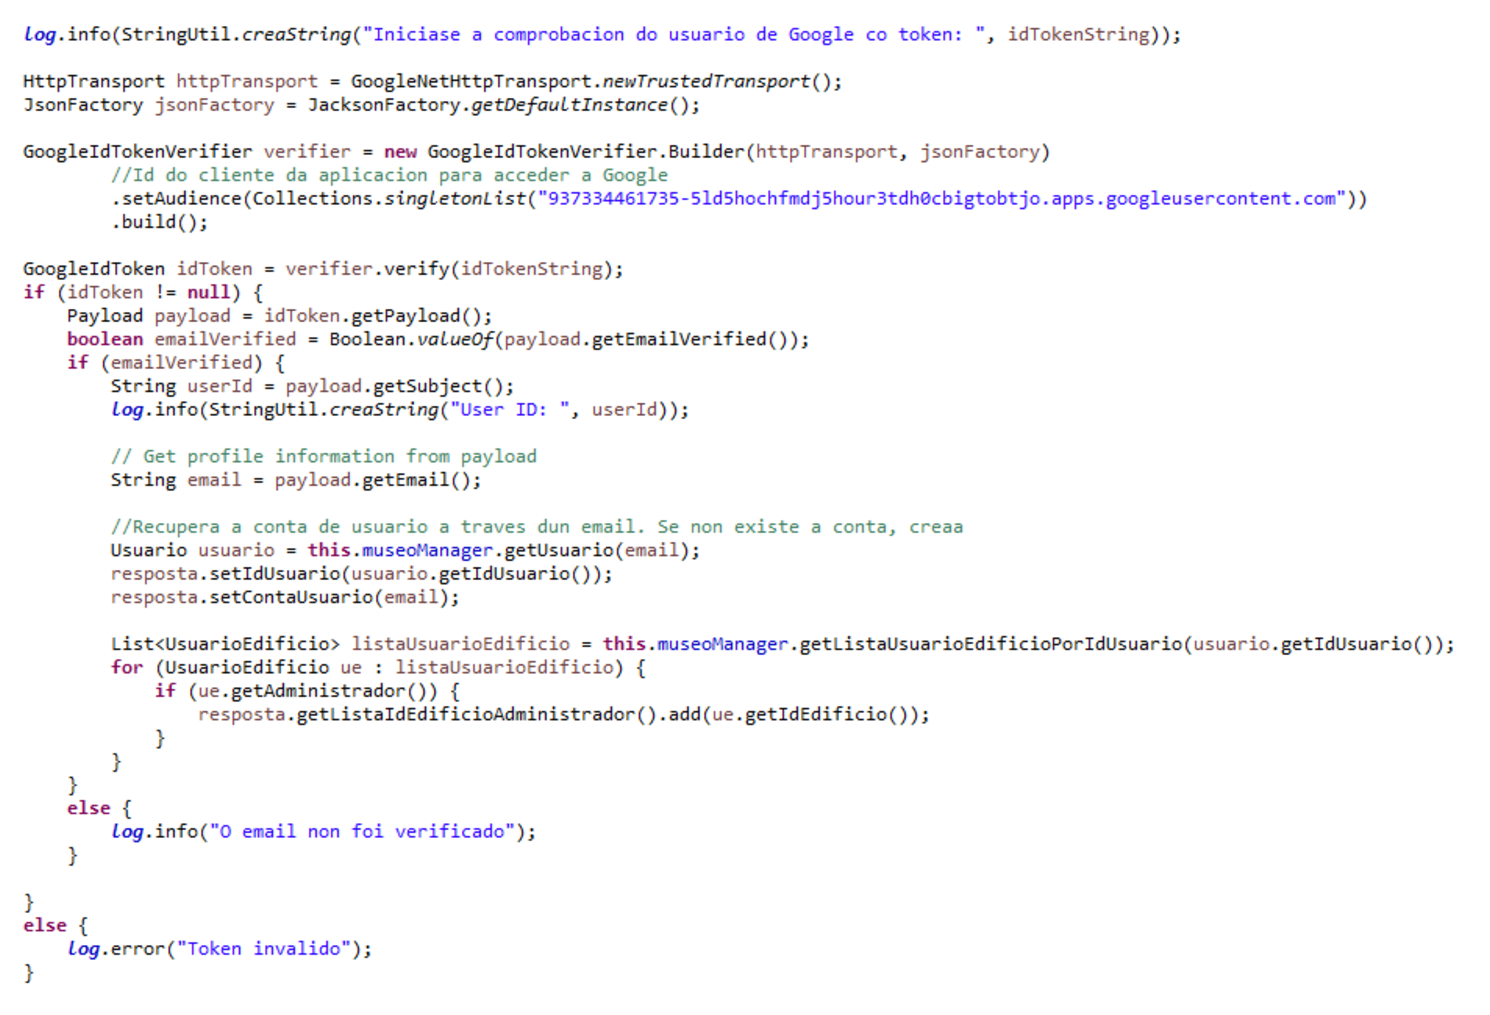
\includegraphics[width=1\textwidth]{figures/codigo/autenticacionGoogleServidor}
		\caption{Código para a autenticación con Google na aplicación (e 3).}
		\label{fig:autenticacionGoogleServidor}
	\end{center}
\end{figure}

Na figura~\ref{fig:autenticacionGoogleServidor} pódese ver o código do servidor co cal se verifica a conta coa que se acaba de autenticar o usuario. Utilízase a clase GoogleIdTokenVerifier para verificar o token recibido na aplicación Android. Se o token é válido, devólvese a información do usuario xunto cos seus roles á aplicación Android, se ten algún. Se é a primeira vez que o usuario accede ao sistema, gardarase a súa conta na base de datos.

Para que funcione a autenticación desde unha aplicación descargada de Google Play débese incluír a chave do certificado co que se firma a aplicación na consola para desenvolvedores de Google.

\todo{Para publicar a aplicación na Play Store}
\todo{https://developer.android.com/studio/publish/app-signing}
